\section{Analisi dati}

Come anticipato nell'introduzione in ottica la legge di Lambert-Beer, conosciuta anche come legge di Beer-Lambert-Bouguer, è una relazione empirica che correla la quantità di luce assorbita da un mezzo alla natura chimica, alla concentrazione ed allo spessore del mezzo attraversato.
Quando un fascio di luce (monocromatica) di intensità $I_0$ attraversa uno strato di spessore $L$ di un mezzo (una soluzione nel nostro caso), una parte di questa intensità viene assorbita dal mezzo stesso e una parte viene trasmessa con intensità residua $I_f$.
In questa breve descrizione del processo abbiamo omesso di considerare che una parte della radiazione luminosa subisce anche effetti di riflessione a causa della pareti del contenitore.

\begin{wrapfigure}{l}{60mm}
    \vspace{-8mm}
    \begin{center}
        
\includegraphics[width=58mm]{doge.pdf}
    \end{center}
    \vspace{-4mm}
\end{wrapfigure}

Quindi il rapporto tra le intensità della luce trasmessa ($I_f$) e incidente ($I_0$) è espresso dalla relazione:

\begin{equation}
	I_f \,\,=\,\, I_0 \,\, e^{-kcL}
	\label{eq:intensita}
\end{equation}

dove con $I_0$ indichiamo l'intensità della radiazione incidente sul contenitore, con $L$ indichiamo il cammino geometrico (ovvero lo spessore del contenitore) e $c$ indica la molarità ovvero la concentrazione di CuSO$_4$ presente nella sostanza (moli su litro). Infine con il termine $k$ indichiamo l'estinzione molare o il coefficiente di assorbimento molare. Ricordiamo che il suo valore è quasi costante per una certa sostanza ad una data lunghezza d'onda, tuttavia può subire lievi variazioni con la temperatura, che noi trascureremo.

Facciamo notare che, nel nostro caso, $I_0$ fa riferimento al valore di intensità della radiazione nel caso in cui nella provetta ci sia solamente acqua distillata, che consideriamo perfettamente trasparente. Poiché abbiamo misurato direttamente questo valore,
quando faremo il fit sui restanti dati potremo controllare che il valore misurato direttamente sia compatibile con quello ricavato dal fit.
Quindi il valore di $I_0$ che ci aspettiamo è:

\begin{equation}
	I_{0\ped{exp}} \,\,=\,\, I\ped{H_2O} \,\,=\,\, 114 \pm 1 \,\,\, \text{rPdtc}
\end{equation}

\subsection{Intensità in funzione della concentrazione molare}

In questa sezione verificheremo se $I\ped{0\ped{exp}}$ risulta essere compatibile col valore di $I_0$ che troveremo dall'analisi dati.
Durante l'esperimento $L$ è stata mantenuta costante, mentre abbiamo variato $c$, che diventa quindi la variabile dell'equazione
(\ref{eq:intensita}). Facciamo il logaritmo della relazione (\ref{eq:intensita}) per poi poterne fare un fit lineare:

\begin{equation}
	\log{I_f} \,\,=\,\, A \,-\, B \, c \qquad \text{dove} \qquad A \,=\, \log{I_0} \quad \text{e} \quad B\,=\, kL
	\label{eq:fit}
\end{equation}

Mediante un fit sulla legge lineare appena trovata siamo in in grado di stimare i valori dei parametri
$A$ e $B$. Il fit sopracitato è riportato in Figura (\ref{fig:g1}). Dal fit lineare abbiamo trovato i seguenti valori per $A$ e $B$:

\begin{equation*}
	A \,=\, 4.72 \pm 0.02 \qquad \text{e} \qquad B \,=\, 2.71 \pm 0.06
\end{equation*}

A questo punto, facendo l'esponenziale di entrambi i membri della formula (\ref{eq:fit}) per tornare alla (\ref{eq:intensita}),
otteniamo che i valori di $I\ped{0}$ e di $kL$ sono i seguenti:

\begin{equation}
	I\ped{0} \,=\, 112 \pm 2 \;\, \text{rPdtc} \qquad \text{e} \qquad kL = B \,=\, 2.71 \pm 0.06
\end{equation}

Quindi il valore delle due intensità $I_0$ e $I\ped{0\ped{exp}}$ risultano essere compatibili entro i loro errori sperimentali. Come si può evincere sia dai dati ottenuti che dall'analisi del grafico in Figura (\ref{fig:g1}) i risultati sono buoni.

\begin{SCfigure}
    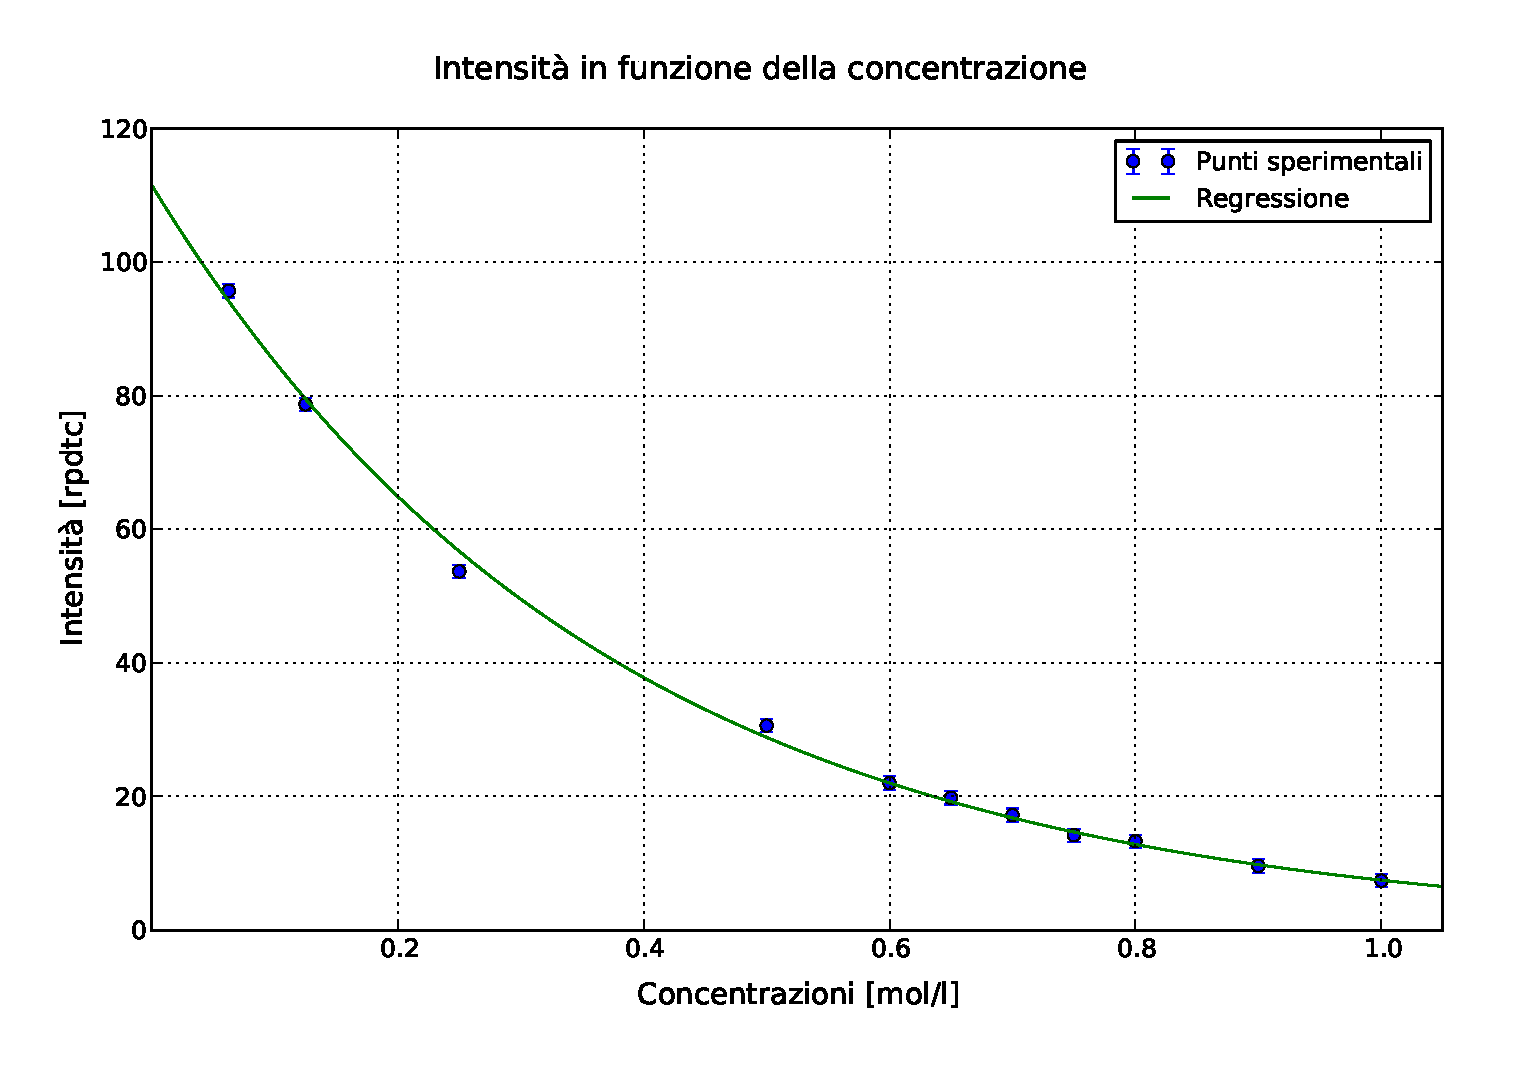
\includegraphics[width=135mm]{g1.pdf}
    \caption{I punti indicano i dati che abbiamo misurato, mentre la linea rappresenta il fit eseguito su di essi.
        Le barre d'errore sono piccole ma visibili (poco più grandi dei punti). Il chi quadro è compatibile entro poco più di un sigma
        con il suo valore teorico. In definitiva la legge ricavata è soddisfacente ed è in buon accordo con i dati.}
    \label{fig:g1}
\end{SCfigure}

\subsection{Intensità in funzione della lunghezza}

Uno dei gruppi di laboratorio ha misurato l'intensità in funzione della lunghezza $L$ si soluzione attraversata dal laser.
La procedura usata non è descritta in dettaglio in questa relazione poichè non è stata eseguita da noi ma da un altro gruppo.
Anche in questo caso è stato misurato un valore di intensità $I_{0\ped{exp}} = 111 \pm 1$ rPdtc che si misura quando il contenitore è vuoto,
cioè quando $L = 0$.
Come nella precedente, in questa sezione ci proponiamo di verificare se $I_{0\ped{exp}}$ risulta essere compatibile col valore di $I\ped{0}$ che troveremo dall'analisi dati. L'unica differenza è che in questo caso la variabile dell'equazione (\ref{eq:intensita}) è $L$, cioè lo spessore del contenitore della sostanza. La concentrazione molare in questo caso è stata mantenuta costante.

Quindi, in maniera analoga a prima, otteniamo che:

\begin{equation}
	\log{I_f} \,\,=\,\, A \,-\, B \, L \qquad \text{dove} \qquad A \,=\, \log{I_0} \quad \text{e} \quad B\,=\, kc
\end{equation}

I valori trovati dalla procedura di fit sulla relazione soprariportata sono:

\begin{center}
\vspace{-2mm}
\begin{tabular}{c c}
	$A \,=\, 4.73 \pm 0.02$ & $B \,=\, 0.037 \pm 0.001$ \\
	$I\ped{0} \,=\, 113 \pm 3$ & $kL = B \,=\, 0.037 \pm 0.001$ \\
\end{tabular}
\vspace{-2mm}
\end{center}

\begin{SCfigure}[1][b!]
    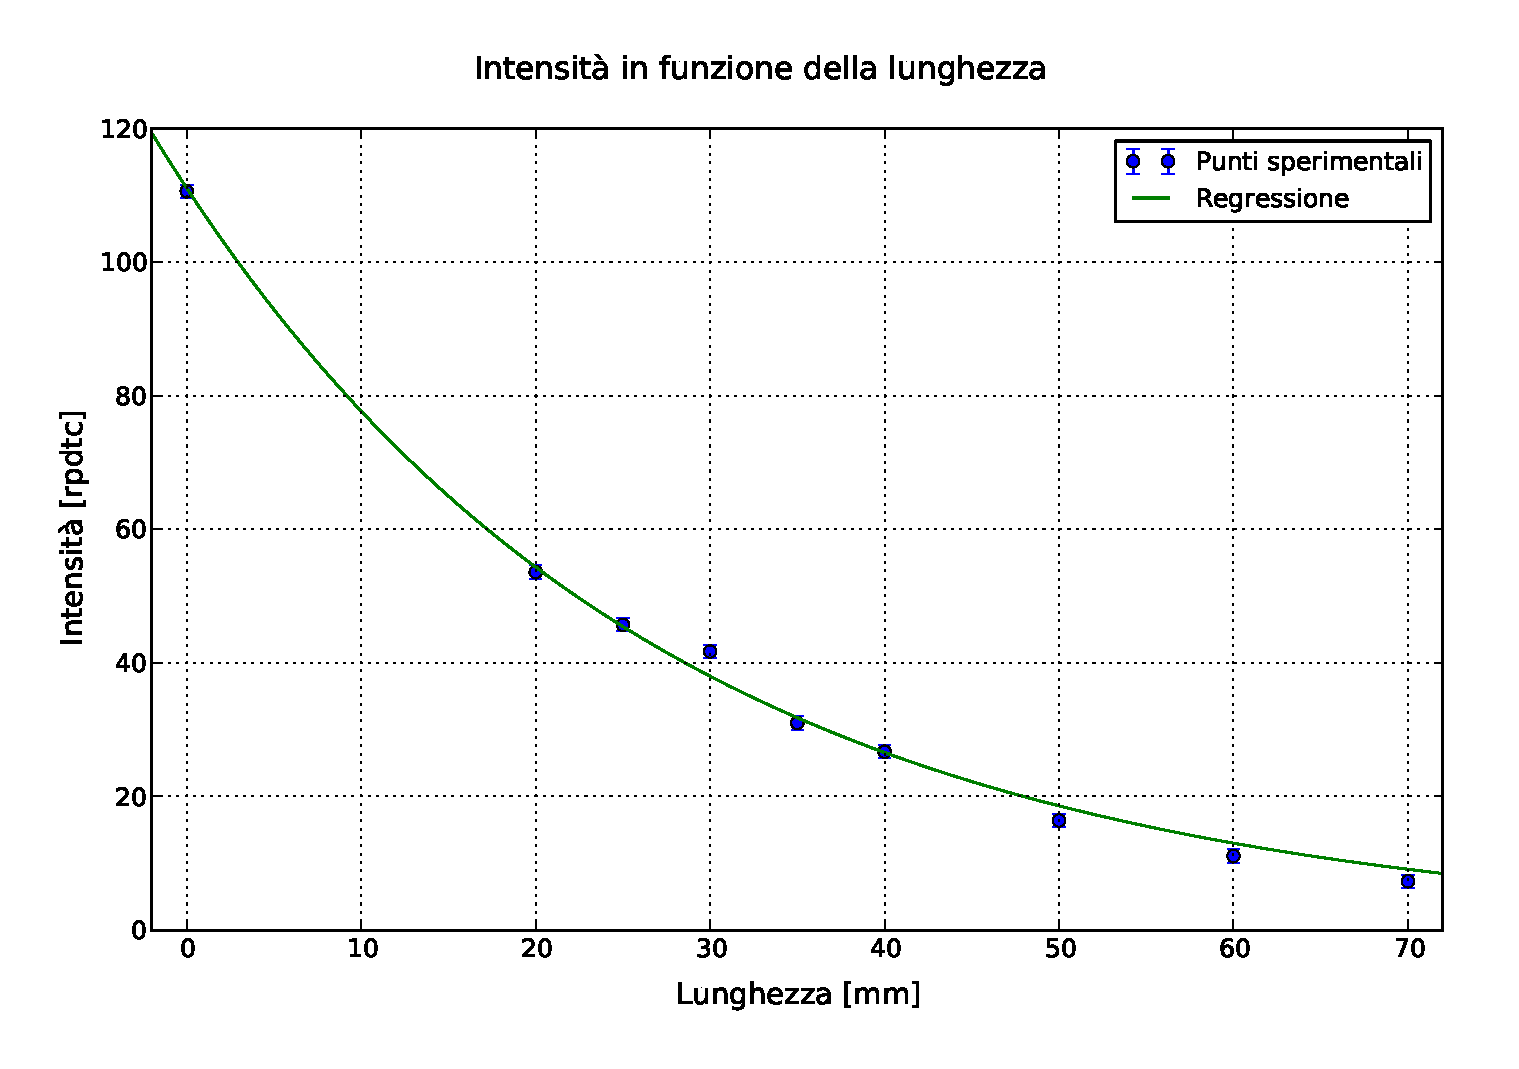
\includegraphics[width=135mm]{g2.pdf}
    \caption{I punti sperimentali e la legge da essi ricavata sono soddisfacenti. Le incertezze sono piccole (appena visibili),
        tuttavia il chi quadro è compatibile con il suo valore teorico.}
    \label{fig:g2}
\end{SCfigure}

Evidentemente anche in questo caso i valori di $I_0$ e $I\ped{0\ped{exp}}$ risultano essere compatibili entro i loro errori sperimentali.
Il grafico in Figura \ref{fig:g2} mostra i dati sperimentali e la legge di fit trovata.
Possiamo dire di aver verificato la legge di Lambert-Beer. Concludiamo augurando Buon Natale e Buone Feste!
